% You should title the file with a .tex extension (hw1.tex, for example)
\documentclass[11pt]{article}

\usepackage{hyperref}
\usepackage{amsmath}
\usepackage{mathtools}
\usepackage{amssymb}
\usepackage{wrapfig}
\usepackage{fancyhdr}
\usepackage{tikz-qtree}
\usepackage{tikz-qtree-compat}
\usepackage[normalem]{ulem}
\usepackage{tikz}
\usepackage{graphicx}
\DeclareMathOperator*{\argmin}{argmin}
\DeclareMathOperator*{\argmax}{argmax}

\oddsidemargin0cm
\topmargin-2cm     %I recommend adding these three lines to increase the 
\textwidth16.5cm   %amount of usable space on the page (and save trees)
\textheight23.5cm  

\newcommand{\question}[2] {\vspace{.25in} \hrule\vspace{0.5em}
\noindent{\bf #1: #2} \vspace{0.5em}
\hrule \vspace{.10in}}
\renewcommand{\part}[1] {\vspace{.10in} {\bf (#1)}}

\newcommand{\myname}{Sean Bittner}
\newcommand{\myandrew}{srb2201@columbia.edu}
\newcommand{\myhwnum}{12}

\setlength{\parindent}{0pt}
\setlength{\parskip}{5pt plus 1pt}
 
\DeclarePairedDelimiter\abs{\lvert}{\rvert}%
 %
\pagestyle{fancyplain}
\rhead{\fancyplain{}{\myname\\ \myandrew}}

\begin{document}

\medskip                        % Skip a "medium" amount of space
                                % (latex determines what medium is)
                                % Also try: \bigskip, \littleskip

\thispagestyle{plain}
\begin{center}                  % Center the following lines
{\Large Inverting nonlinear systems with approximately Bernoulli responses} \\
Sean Bittner \\
April 4, 2019 \\
\end{center}

\section{Introduction}
We want to have approximately Bernoulli responses of the SC network in the various conditions.  Before modeling the full task, we should figure out the appropriate way to invert a nonlinear dynamical system with approx. Bernoulli responses in a single condition.  The key question is how to model this ``emergent property" as a moment constraint.  

\section{SC Model}
There are four total units: two in each hemisphere corresponding to the PRO/CONTRA and ANTI/IPSI populations.  Each unit had an external ($V_i$) and internal ($U_i$) variable related by
\begin{equation}
V_i(t) =\eta(t)\left(\frac{1}{2}\tanh\left(\frac{U_i(t) - \theta}{\beta}\right)+ \frac{1}{2} \right)
\end{equation}
$\theta = 0.05$ and $\beta = 0.5$ control the position and shape of the nonlinearity, repsectively, and $\eta(t)$ is the optogenetic inactivation function.

We can order the elements of $V_i$ and $U_i$ into vectors $v$ and $u$ with elements
\begin{equation}
v = \begin{bmatrix} V_{LP} \\ V_{LA} \\ V_{RA} \\ V_{RP} \end{bmatrix} \hspace{2cm} u = \begin{bmatrix} U_{LP} \\ U_{LA} \\ U_{RA} \\ U_{RP} \end{bmatrix}
\end{equation}

 The internal variables follow dynamics:
\begin{equation}
\tau \frac{\partial u}{\partial t} = -u + Wv + I + \sigma \partial W
\end{equation}
with time constant $\tau = 0.09s$ and gaussian noise $\sigma \partial W$ controlled by the magnitude of $\sigma$.  The weight matrix has 8 parameters $sW_P$, $sW_A$, $vW_{PA}$, $vW_{AP}$, $hW_P$, $hW_A$, $dW_{PA}$, and $dW_{AP}$,  related to the depiction in Fig. 2:
\begin{center}
\textbf{Full Model} \\
\end{center}
\begin{equation}
W = \begin{bmatrix} sW_P & vW_{PA} &  dW_{PA} & hW_P \\ vW_{AP}  & sW_A & hW_A  & dW_{AP} \\ dW_{AP} & hW_P & sW_A & vW_{AP}  \\  hW_A & dW_{PA} & vW_{PA}  & sW_P \end{bmatrix}
\end{equation}

The input is a sum of five task-relalated inputs.
\begin{equation}
I = I_{\text{constant}} + I_{\text{pro-bias}} + I_{\text{rule}} + I_{\text{choice-period}} + I_{\text{light}}
\end{equation}

We'll also consider a 4-parameter reduced model:
\begin{center}
\textbf{Reduced Model} \\
\end{center}
\begin{equation}
W = \begin{bmatrix} sW & vW &  dW & hW \\ vW  & sW & hW  & dW \\ dW & hW & sW & vW \\  hW & dW & vW  & sW \end{bmatrix}
\end{equation}

\section{Setting up the DSN behavior constraints}

Let's say that we want to learn the parameters that produce a Bernoulli rate of $p_{LP}$ in the Left, Pro condition.  We'll let $\hat{p}_i$ be the empirical average steady state (ss) response (final $V_{LP}$ at end of task) over M=100 gaussian noise draws for a given dynamical system parameterization $z_i$:

\begin{equation}
 \hat{p}_i = E_{\sigma \partial W} \left[ V_{LP,\text{ss}} \mid s=L, c=P, z_i \right] = \frac{1}{M}\sum_{j=1}^M V_{LP,\text{ss}}(s=L, c=P, z_i, \sigma \partial W_j)
 \end{equation}

The noise is fixed at $\sigma = 0.3$ (the average of satisfactory parameterizations from Duan et al.).  For the 1st constraint, we certainly want the average over DSN samples to be $p_{LP}$:
\begin{equation}
E_{z \sim q_\phi} \left[ E_{\sigma \partial W} \left[ V_{LP,\text{ss}} \mid s=L, c=P, z \right] \right] = E_{z \sim q_\phi} \left[ \hat{p} \right] = p_{LP}
\end{equation}

We can then ask that the variance of the steady state responses across gaussian draws, is the Bernoulli variance for the empirical rate $\hat{p}$.
\begin{equation}
 Var_{\sigma \partial W} \left[ V_{LP,\text{ss}} \mid s=L, c=P, _iz \right] = \hat{p}(1 - \hat{p})
\end{equation}

With DSNs, we enforce constraints in expectation over DSN samples, so we can force Bernoulli responses with this 2nd constraint:
\begin{equation}
E_{z \sim q\phi} \left[ Var_{\sigma \partial W} \left[ V_{LP,\text{ss}} \mid s=L, c=P, _iz \right] - \hat{p}(1 - \hat{p}) \right] = 0
\end{equation}

Since the maximum variance of a random variable bounded from 0 to 1 is the Bernoulli variance ($\hat{p}(1-\hat{p})$), in principal, we do not need to control the second moment (over DSN samples) of this test-static (the variance over gaussian draws).  In reality, these variables are dynamical system states and can only exponentially decay (or saturate) to 0 (or 1), so the Bernoulli variance constraint can only be undershot.  This is important to be mindful of, when thinking about how to enforce Bernoulli responses in this fashion.

\section{An attempt was made \\(to sample Bernoulli networks)}

\textbf{reduced entropy p = 0.5}
\begin{center}
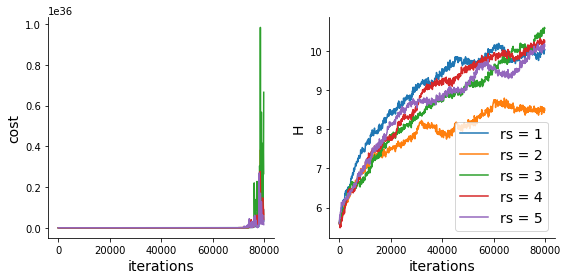
\includegraphics[scale=0.6]{figs/cost_H_SC_reduced_c=15_p=50.png} \\
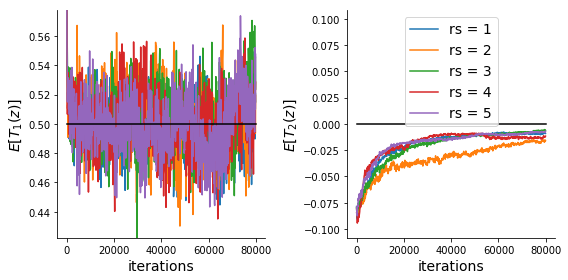
\includegraphics[scale=0.6]{figs/constraints_SC_reduced_c=15_p=50.png}
\end{center}
\begin{center}
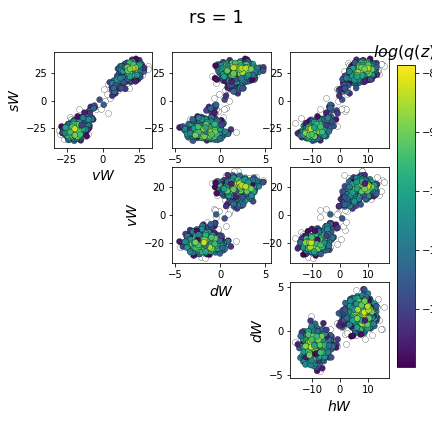
\includegraphics[scale=0.33]{figs/Z_SC_reduced_c=15_p=50_rs=1.png}
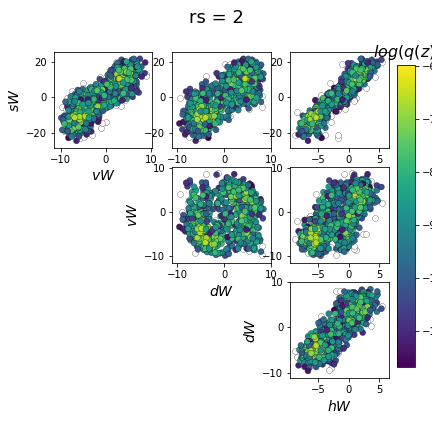
\includegraphics[scale=0.33]{figs/Z_SC_reduced_c=15_p=50_rs=2.png}
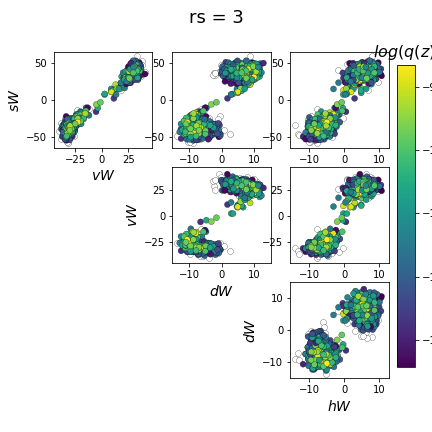
\includegraphics[scale=0.33]{figs/Z_SC_reduced_c=15_p=50_rs=3.png} \\
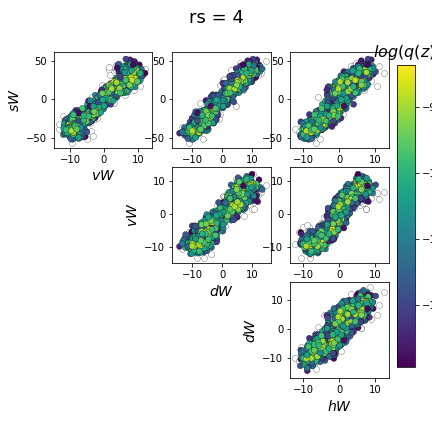
\includegraphics[scale=0.33]{figs/Z_SC_reduced_c=15_p=50_rs=4.png}
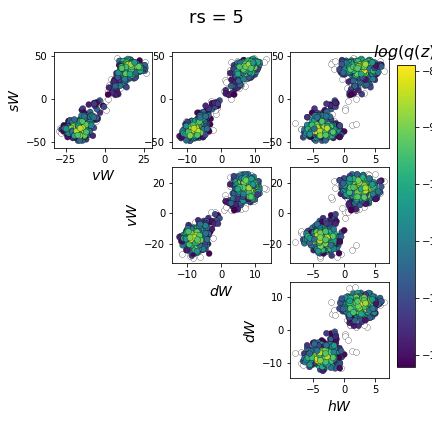
\includegraphics[scale=0.33]{figs/Z_SC_reduced_c=15_p=50_rs=5.png}
\end{center}
\begin{center}
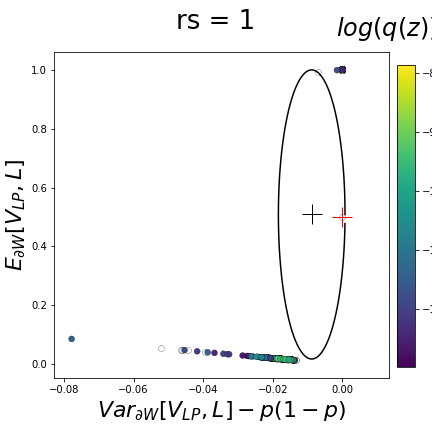
\includegraphics[scale=0.33]{figs/T_x_SC_reduced_c=15_p=50_rs=1.png}
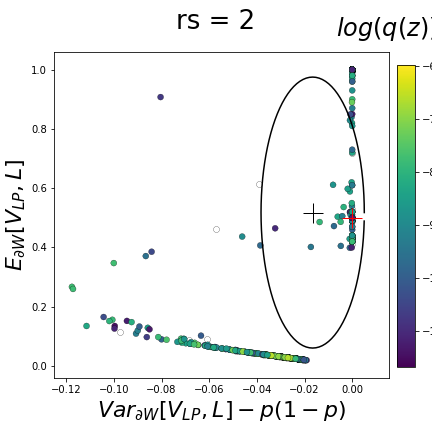
\includegraphics[scale=0.33]{figs/T_x_SC_reduced_c=15_p=50_rs=2.png}
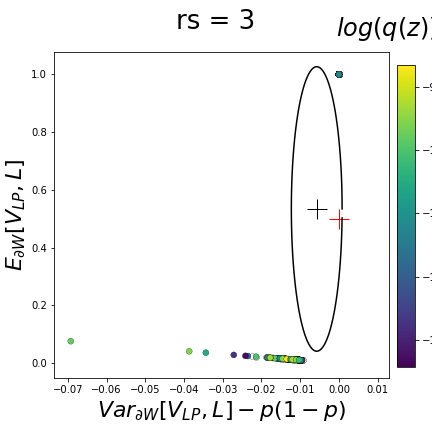
\includegraphics[scale=0.33]{figs/T_x_SC_reduced_c=15_p=50_rs=3.png} \\
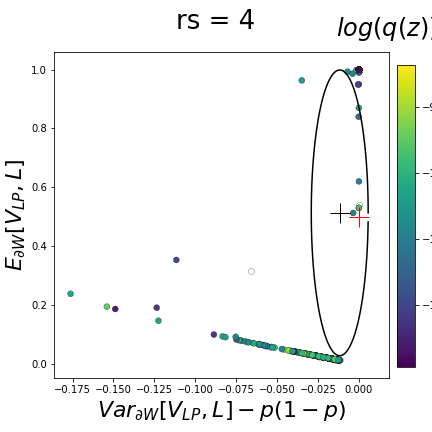
\includegraphics[scale=0.33]{figs/T_x_SC_reduced_c=15_p=50_rs=4.png}
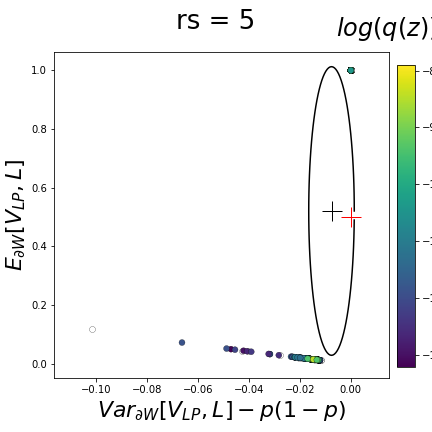
\includegraphics[scale=0.33]{figs/T_x_SC_reduced_c=15_p=50_rs=5.png}
\end{center}



\textbf{reduced NO entropy p = 0.5}
\begin{center}
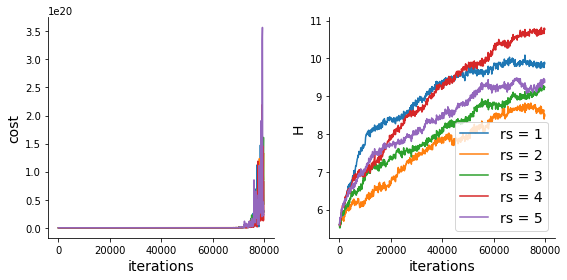
\includegraphics[scale=0.6]{figs/cost_H_SC_reduced_c=0_p=50.png} \\
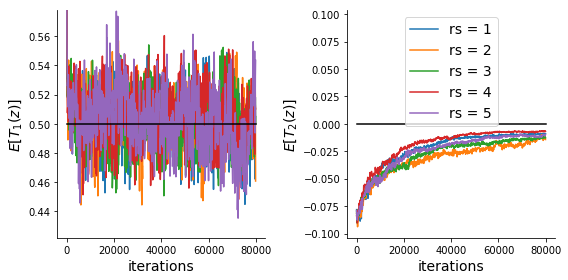
\includegraphics[scale=0.6]{figs/constraints_SC_reduced_c=0_p=50.png}
\end{center}
\begin{center}
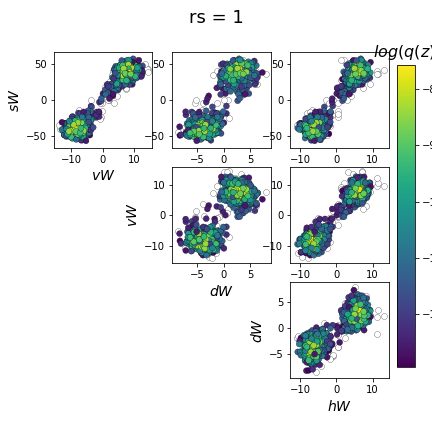
\includegraphics[scale=0.33]{figs/Z_SC_reduced_c=0_p=50_rs=1.png}
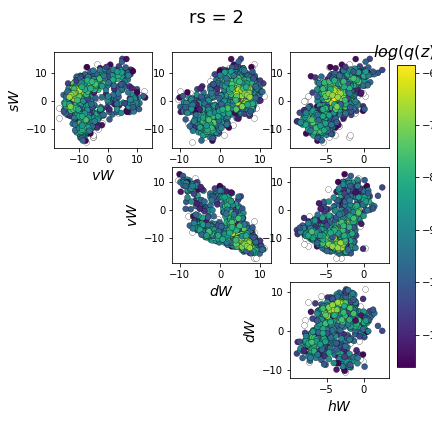
\includegraphics[scale=0.33]{figs/Z_SC_reduced_c=0_p=50_rs=2.png}
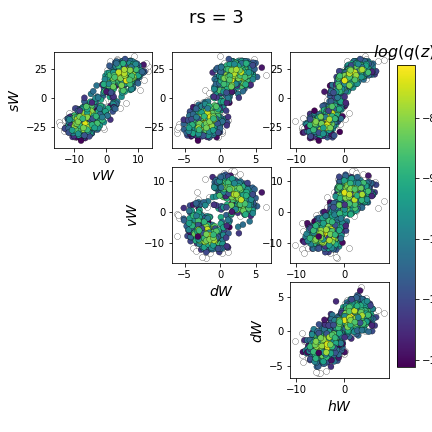
\includegraphics[scale=0.33]{figs/Z_SC_reduced_c=0_p=50_rs=3.png} \\
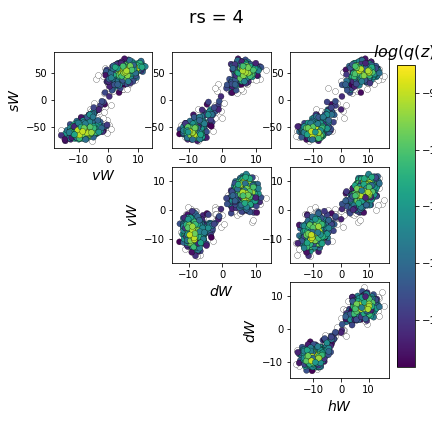
\includegraphics[scale=0.33]{figs/Z_SC_reduced_c=0_p=50_rs=4.png}
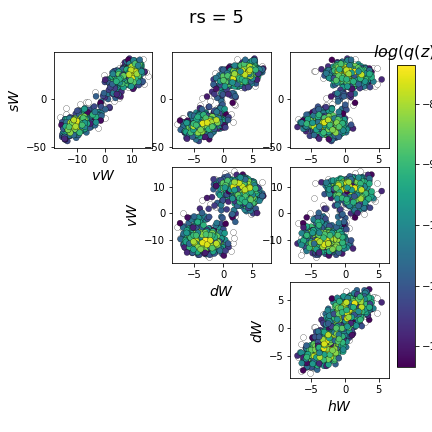
\includegraphics[scale=0.33]{figs/Z_SC_reduced_c=0_p=50_rs=5.png}
\end{center}
\begin{center}
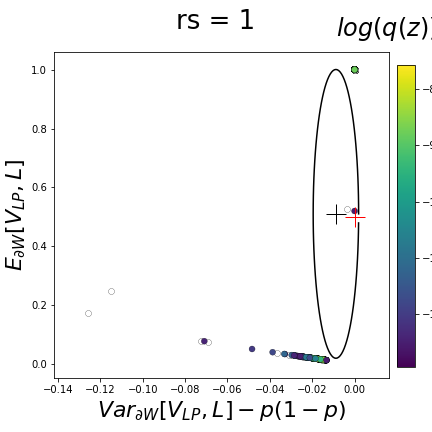
\includegraphics[scale=0.33]{figs/T_x_SC_reduced_c=0_p=50_rs=1.png}
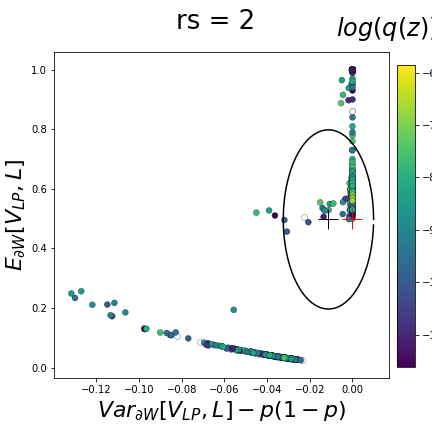
\includegraphics[scale=0.33]{figs/T_x_SC_reduced_c=0_p=50_rs=2.png}
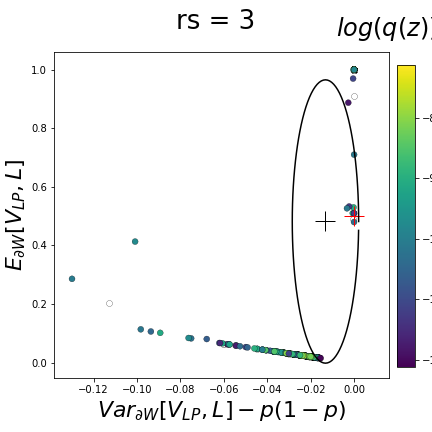
\includegraphics[scale=0.33]{figs/T_x_SC_reduced_c=0_p=50_rs=3.png} \\
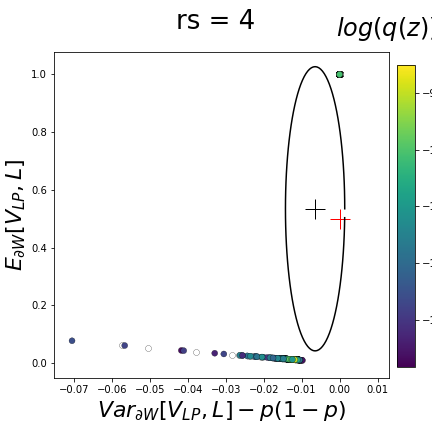
\includegraphics[scale=0.33]{figs/T_x_SC_reduced_c=0_p=50_rs=4.png}
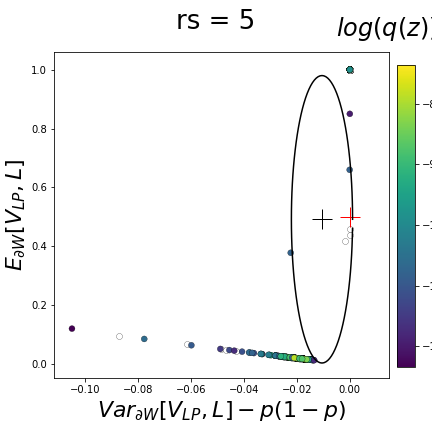
\includegraphics[scale=0.33]{figs/T_x_SC_reduced_c=0_p=50_rs=5.png}
\end{center}


\textbf{full NO entropy p = 0.5}
\begin{center}
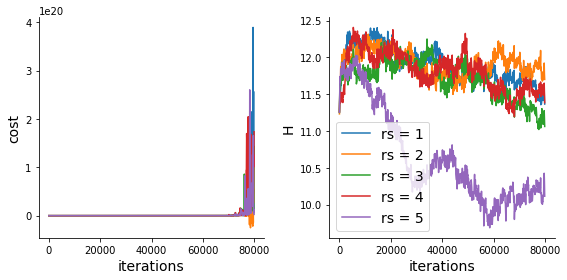
\includegraphics[scale=0.6]{figs/cost_H_SC_full_c=0_p=50.png} \\
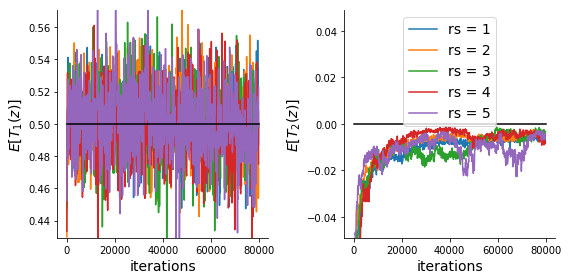
\includegraphics[scale=0.6]{figs/constraints_SC_full_c=0_p=50.png}
\end{center}
\begin{center}
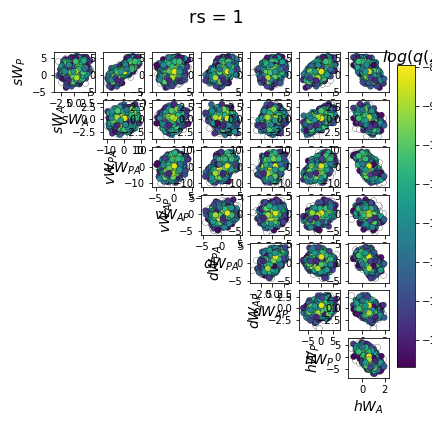
\includegraphics[scale=0.33]{figs/Z_SC_full_c=0_p=50_rs=1.png}
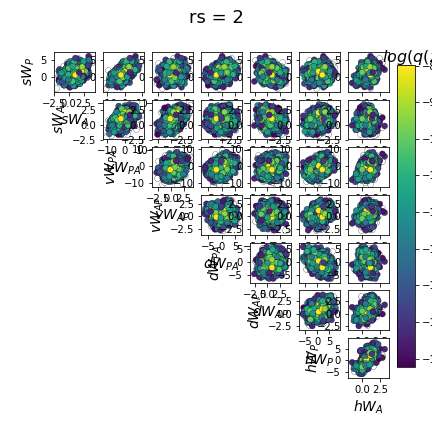
\includegraphics[scale=0.33]{figs/Z_SC_full_c=0_p=50_rs=2.png}
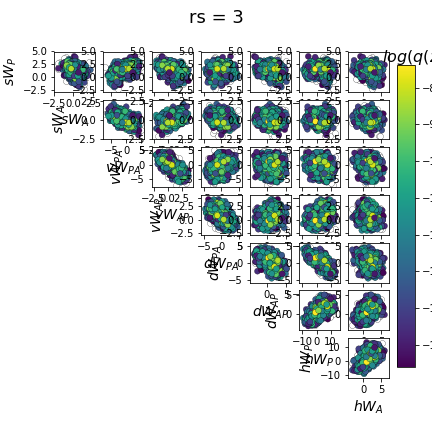
\includegraphics[scale=0.33]{figs/Z_SC_full_c=0_p=50_rs=3.png} \\
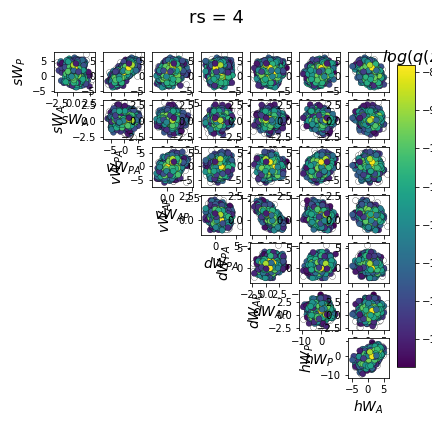
\includegraphics[scale=0.33]{figs/Z_SC_full_c=0_p=50_rs=4.png}
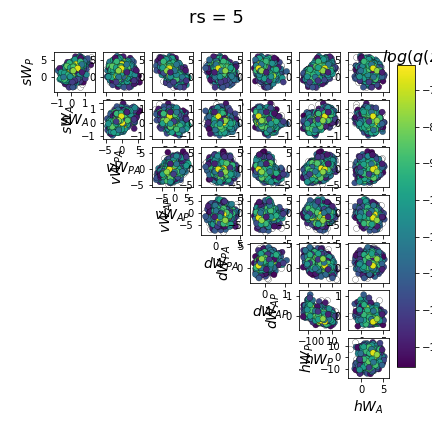
\includegraphics[scale=0.33]{figs/Z_SC_full_c=0_p=50_rs=5.png}
\end{center}
\begin{center}
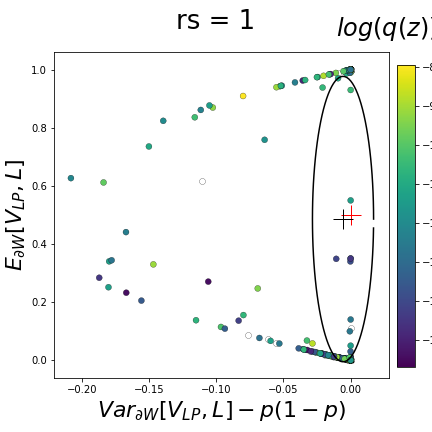
\includegraphics[scale=0.33]{figs/T_x_SC_full_c=0_p=50_rs=1.png}
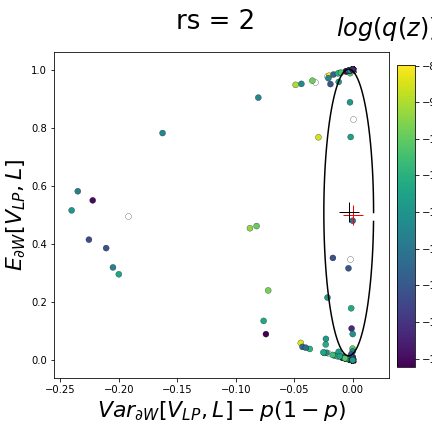
\includegraphics[scale=0.33]{figs/T_x_SC_full_c=0_p=50_rs=2.png}
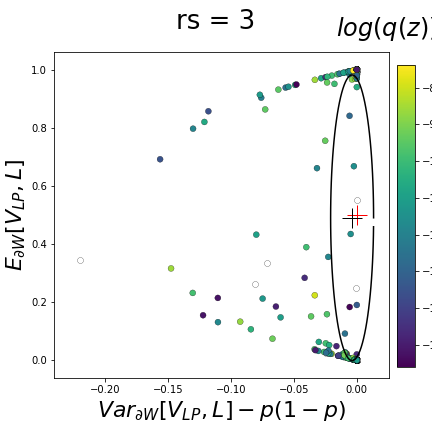
\includegraphics[scale=0.33]{figs/T_x_SC_full_c=0_p=50_rs=3.png} \\
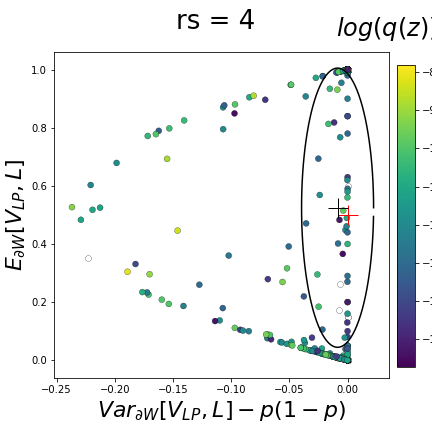
\includegraphics[scale=0.33]{figs/T_x_SC_full_c=0_p=50_rs=4.png}
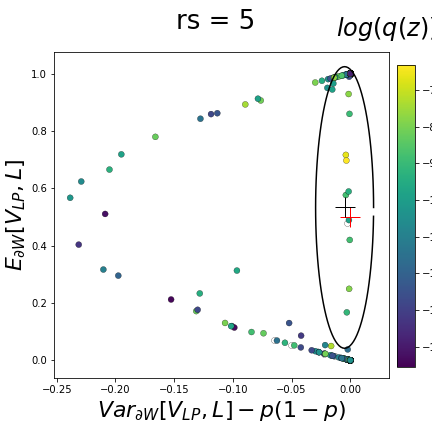
\includegraphics[scale=0.33]{figs/T_x_SC_full_c=0_p=50_rs=5.png}
\end{center}


\textbf{full NO entropy p = 0.8}
\begin{center}
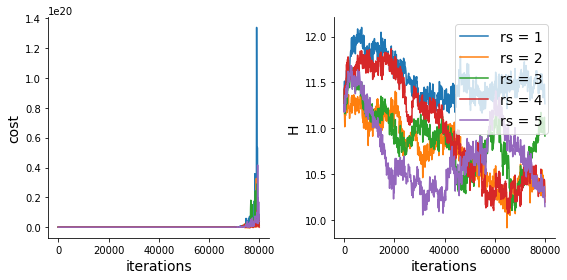
\includegraphics[scale=0.6]{figs/cost_H_SC_full_c=0_p=80.png} \\
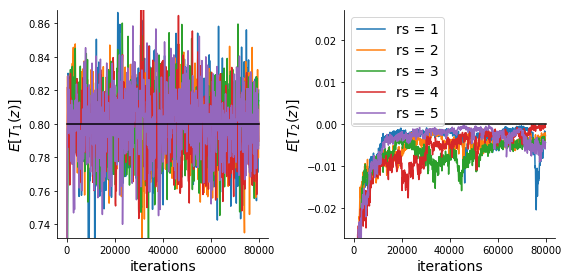
\includegraphics[scale=0.6]{figs/constraints_SC_full_c=0_p=80.png}
\end{center}
\begin{center}
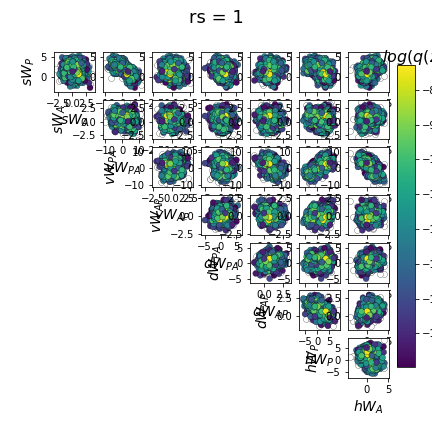
\includegraphics[scale=0.33]{figs/Z_SC_full_c=0_p=80_rs=1.png}
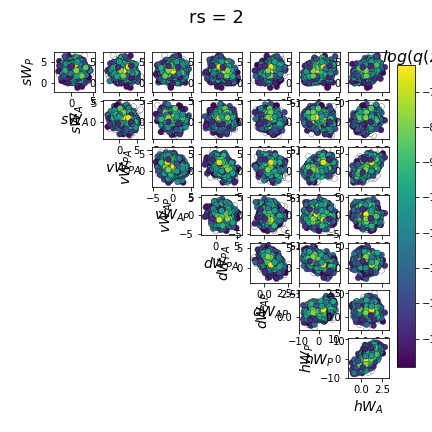
\includegraphics[scale=0.33]{figs/Z_SC_full_c=0_p=80_rs=2.png}
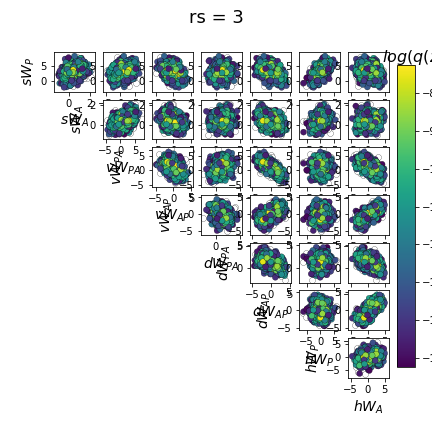
\includegraphics[scale=0.33]{figs/Z_SC_full_c=0_p=80_rs=3.png} \\
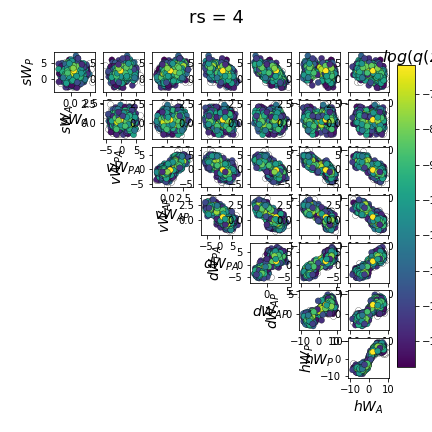
\includegraphics[scale=0.33]{figs/Z_SC_full_c=0_p=80_rs=4.png}
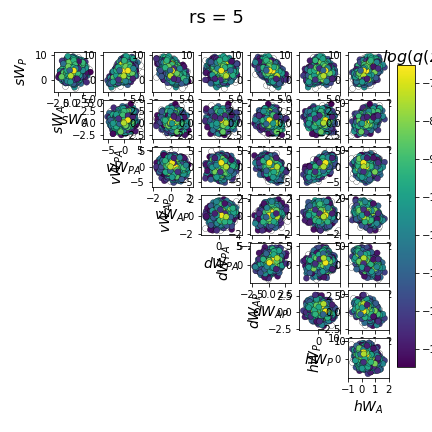
\includegraphics[scale=0.33]{figs/Z_SC_full_c=0_p=80_rs=5.png}
\end{center}
\begin{center}
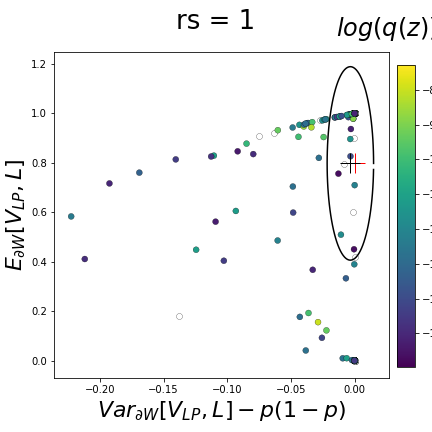
\includegraphics[scale=0.33]{figs/T_x_SC_full_c=0_p=80_rs=1.png}
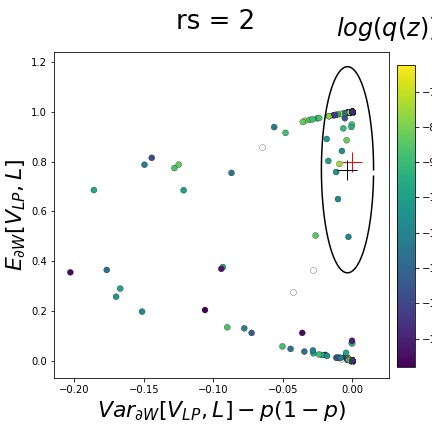
\includegraphics[scale=0.33]{figs/T_x_SC_full_c=0_p=80_rs=2.png}
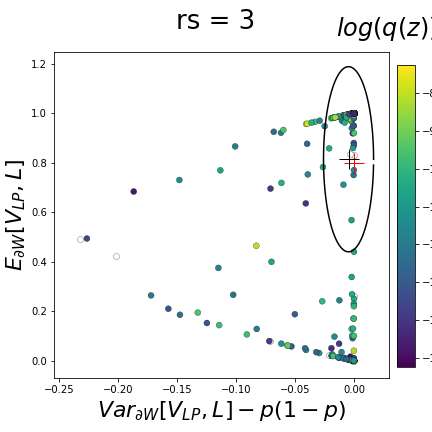
\includegraphics[scale=0.33]{figs/T_x_SC_full_c=0_p=80_rs=3.png} \\
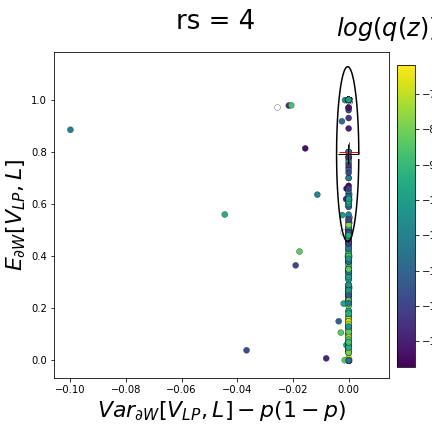
\includegraphics[scale=0.33]{figs/T_x_SC_full_c=0_p=80_rs=4.png}
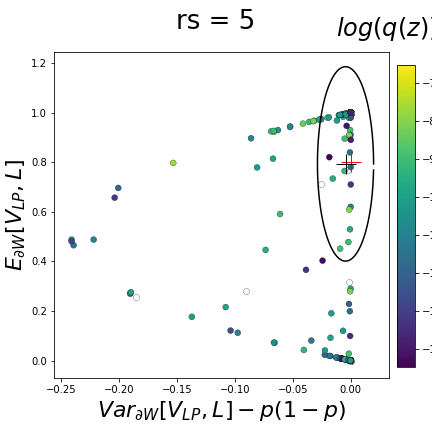
\includegraphics[scale=0.33]{figs/T_x_SC_full_c=0_p=80_rs=5.png}
\end{center}

\bibliography{dsn}
\bibliographystyle{unsrt}

\end{document}

